\section{Architettura software}
L'applicazione mobile di \textbf{FitTag} è sviluppata in linguaggio Dart sfruttando il framework \textbf{Flutter}. 
Questa scelta tecnologica consente di mantenere un'unica base di codice per le piattaforme Android e iOS, garantendo al contempo prestazioni native e un'interfaccia utente altamente responsiva e personalizzata.

L'infrastruttura dell'applicazione si basa su una progettazione guidata dagli eventi, strutturata sui seguenti componenti principali:
\begin{itemize}
    \item \textbf{Gestione dello stato:} implementata secondo un modello reattivo in cui un modulo centrale funge da unica sorgente di verità per l'interfaccia utente, esponendo lo stato di connessione, i dati di telemetria dell'allenamento attivo, i risultati di inferenza in tempo reale, l'età dell'utente e lo storico delle sessioni passate. I componenti grafici si aggiornano in modo automatico solo al variare dei dati di loro interesse.
    \item \textbf{Hardware abstraction layer:} La comunicazione wireless a basso consumo è delegata ad un modulo specifico che si occupa delle operazioni a basso livello sullo stack BLE: la scansione per l'individuazione del bracciale, la connessione fisica e logica, la ricerca dei servizi GATT, la lettura/scrittura di caratteristiche e la sottoscrizione ai canali di notifica asincroni.
    \item \textbf{Persistenza dei dati:} Le sessioni di allenamento completate e le preferenze dell'utente (come l'età) vengono salvate localmente nella memoria non volatile del dispositivo mobile. Questo evita la necessità di un database complesso, garantendo la totale privacy dei dati dell'utente e la disponibilità offline dello storico.
    \item \textbf{Visualizzazione biometrica:} La rappresentazione grafica delle metriche sportive è affidata ad una libreria dedicata che consente di visualizzare grafici temporali a linee con tooltip interattivi attivati al tocco.
\end{itemize}

\begin{figure}[ht]
    \centering
    \begin{subfigure}[t]{0.3\textwidth}
        \centering
        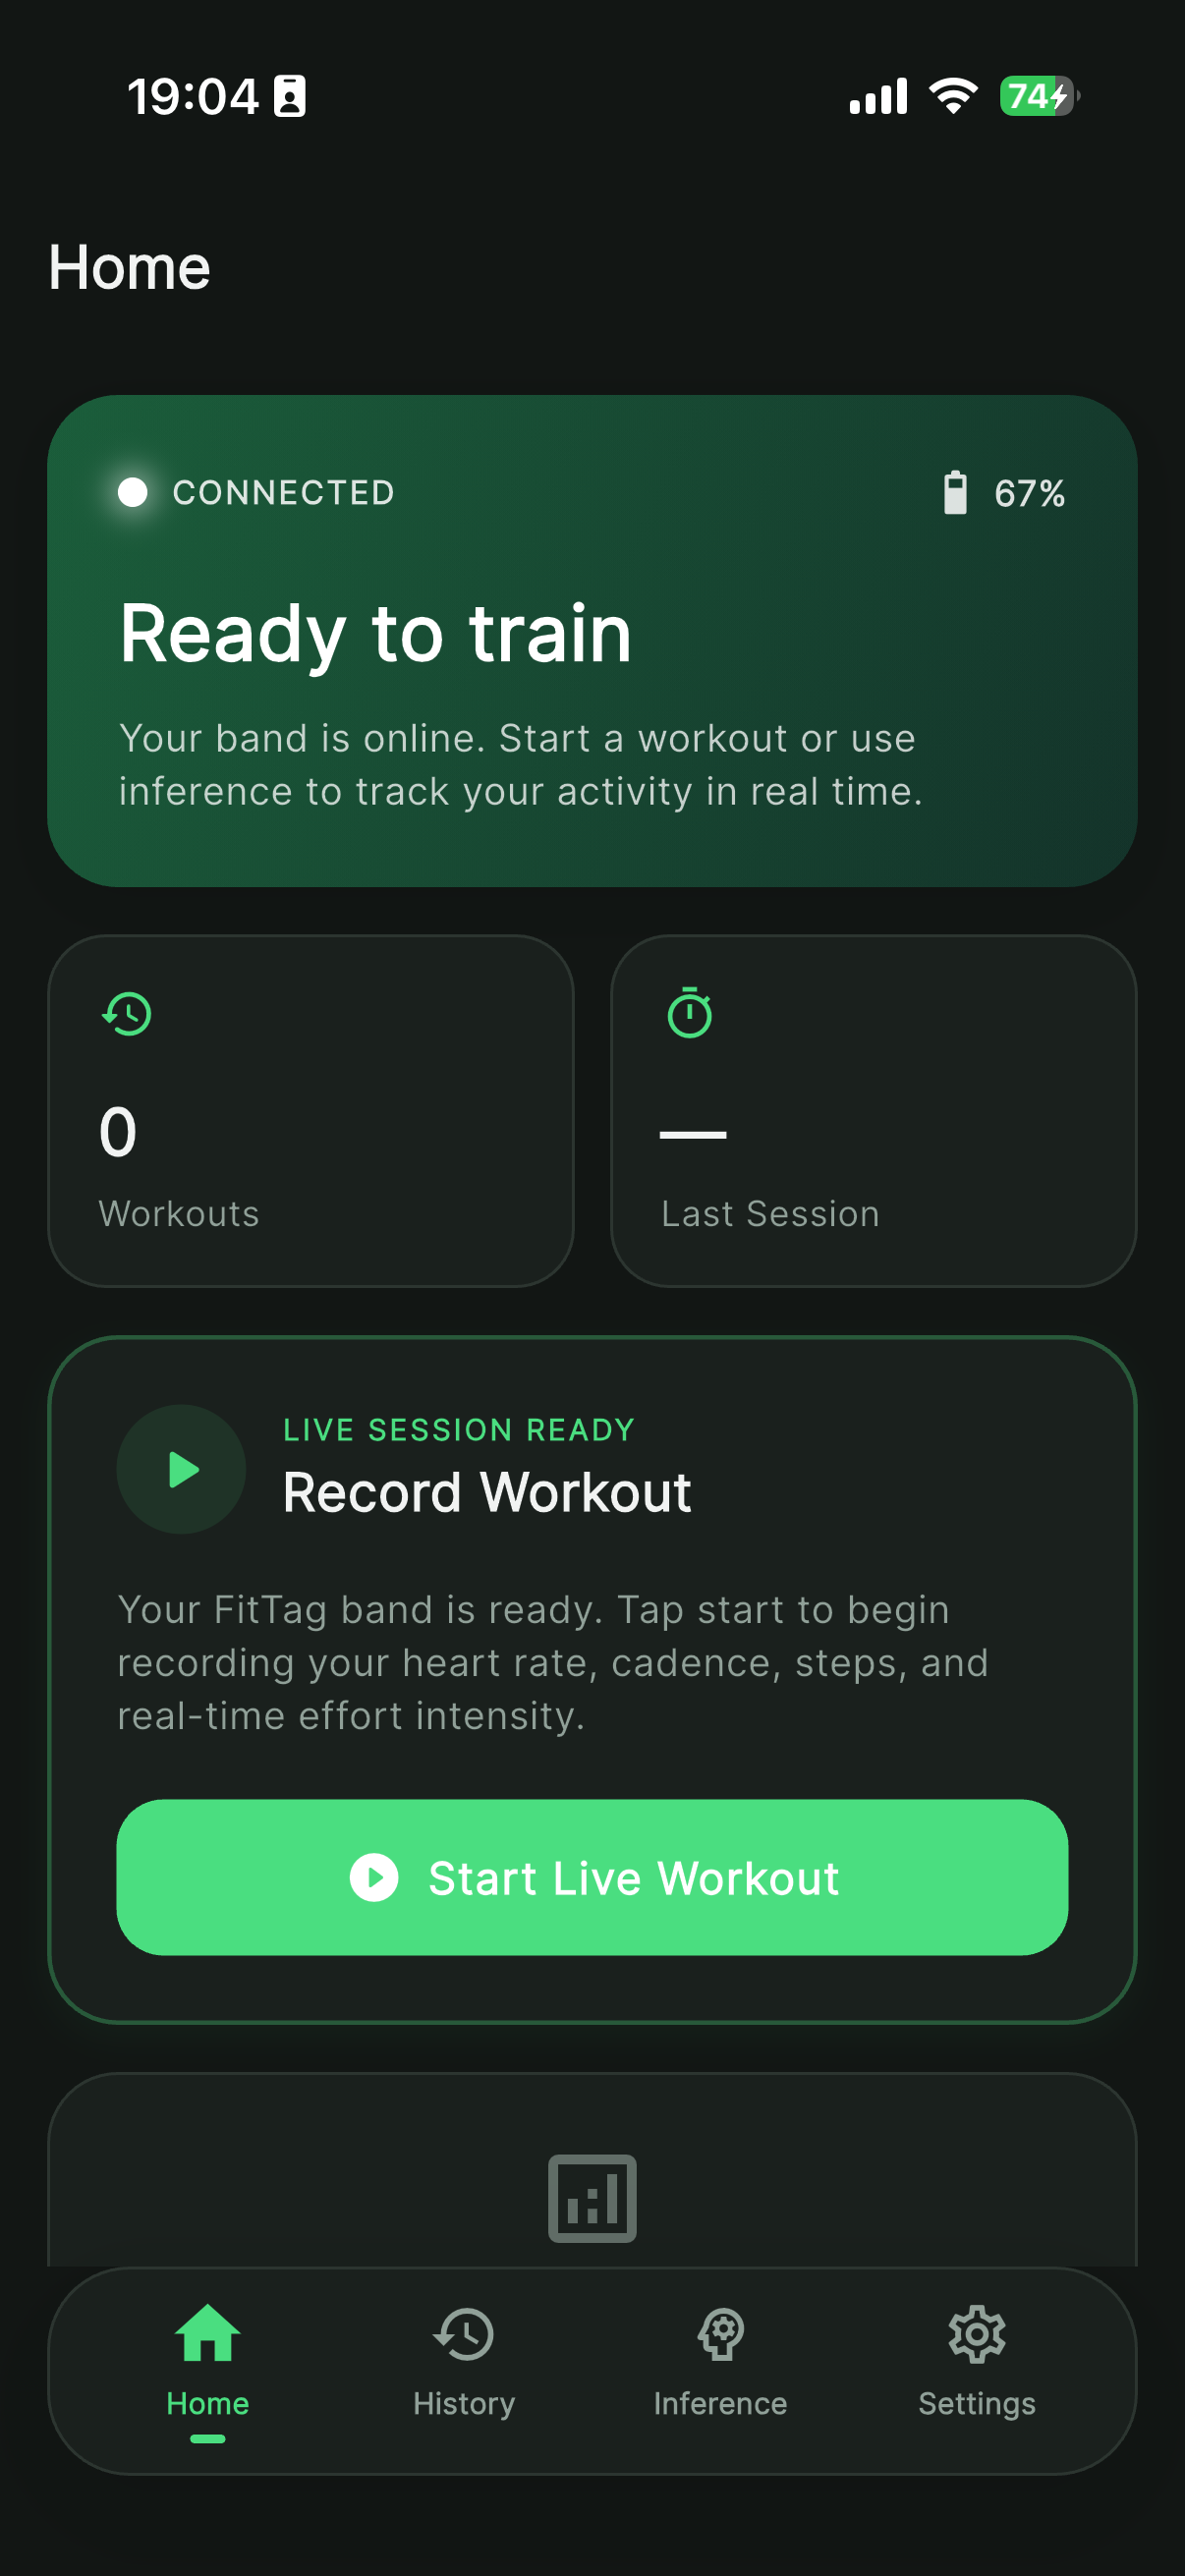
\includegraphics[width=\textwidth]{img/app/home_screen.png}
        \caption{Home Screen}
        \label{fig:home_screen}
    \end{subfigure}
    \hfill
    \begin{subfigure}[t]{0.3\textwidth}
        \centering
        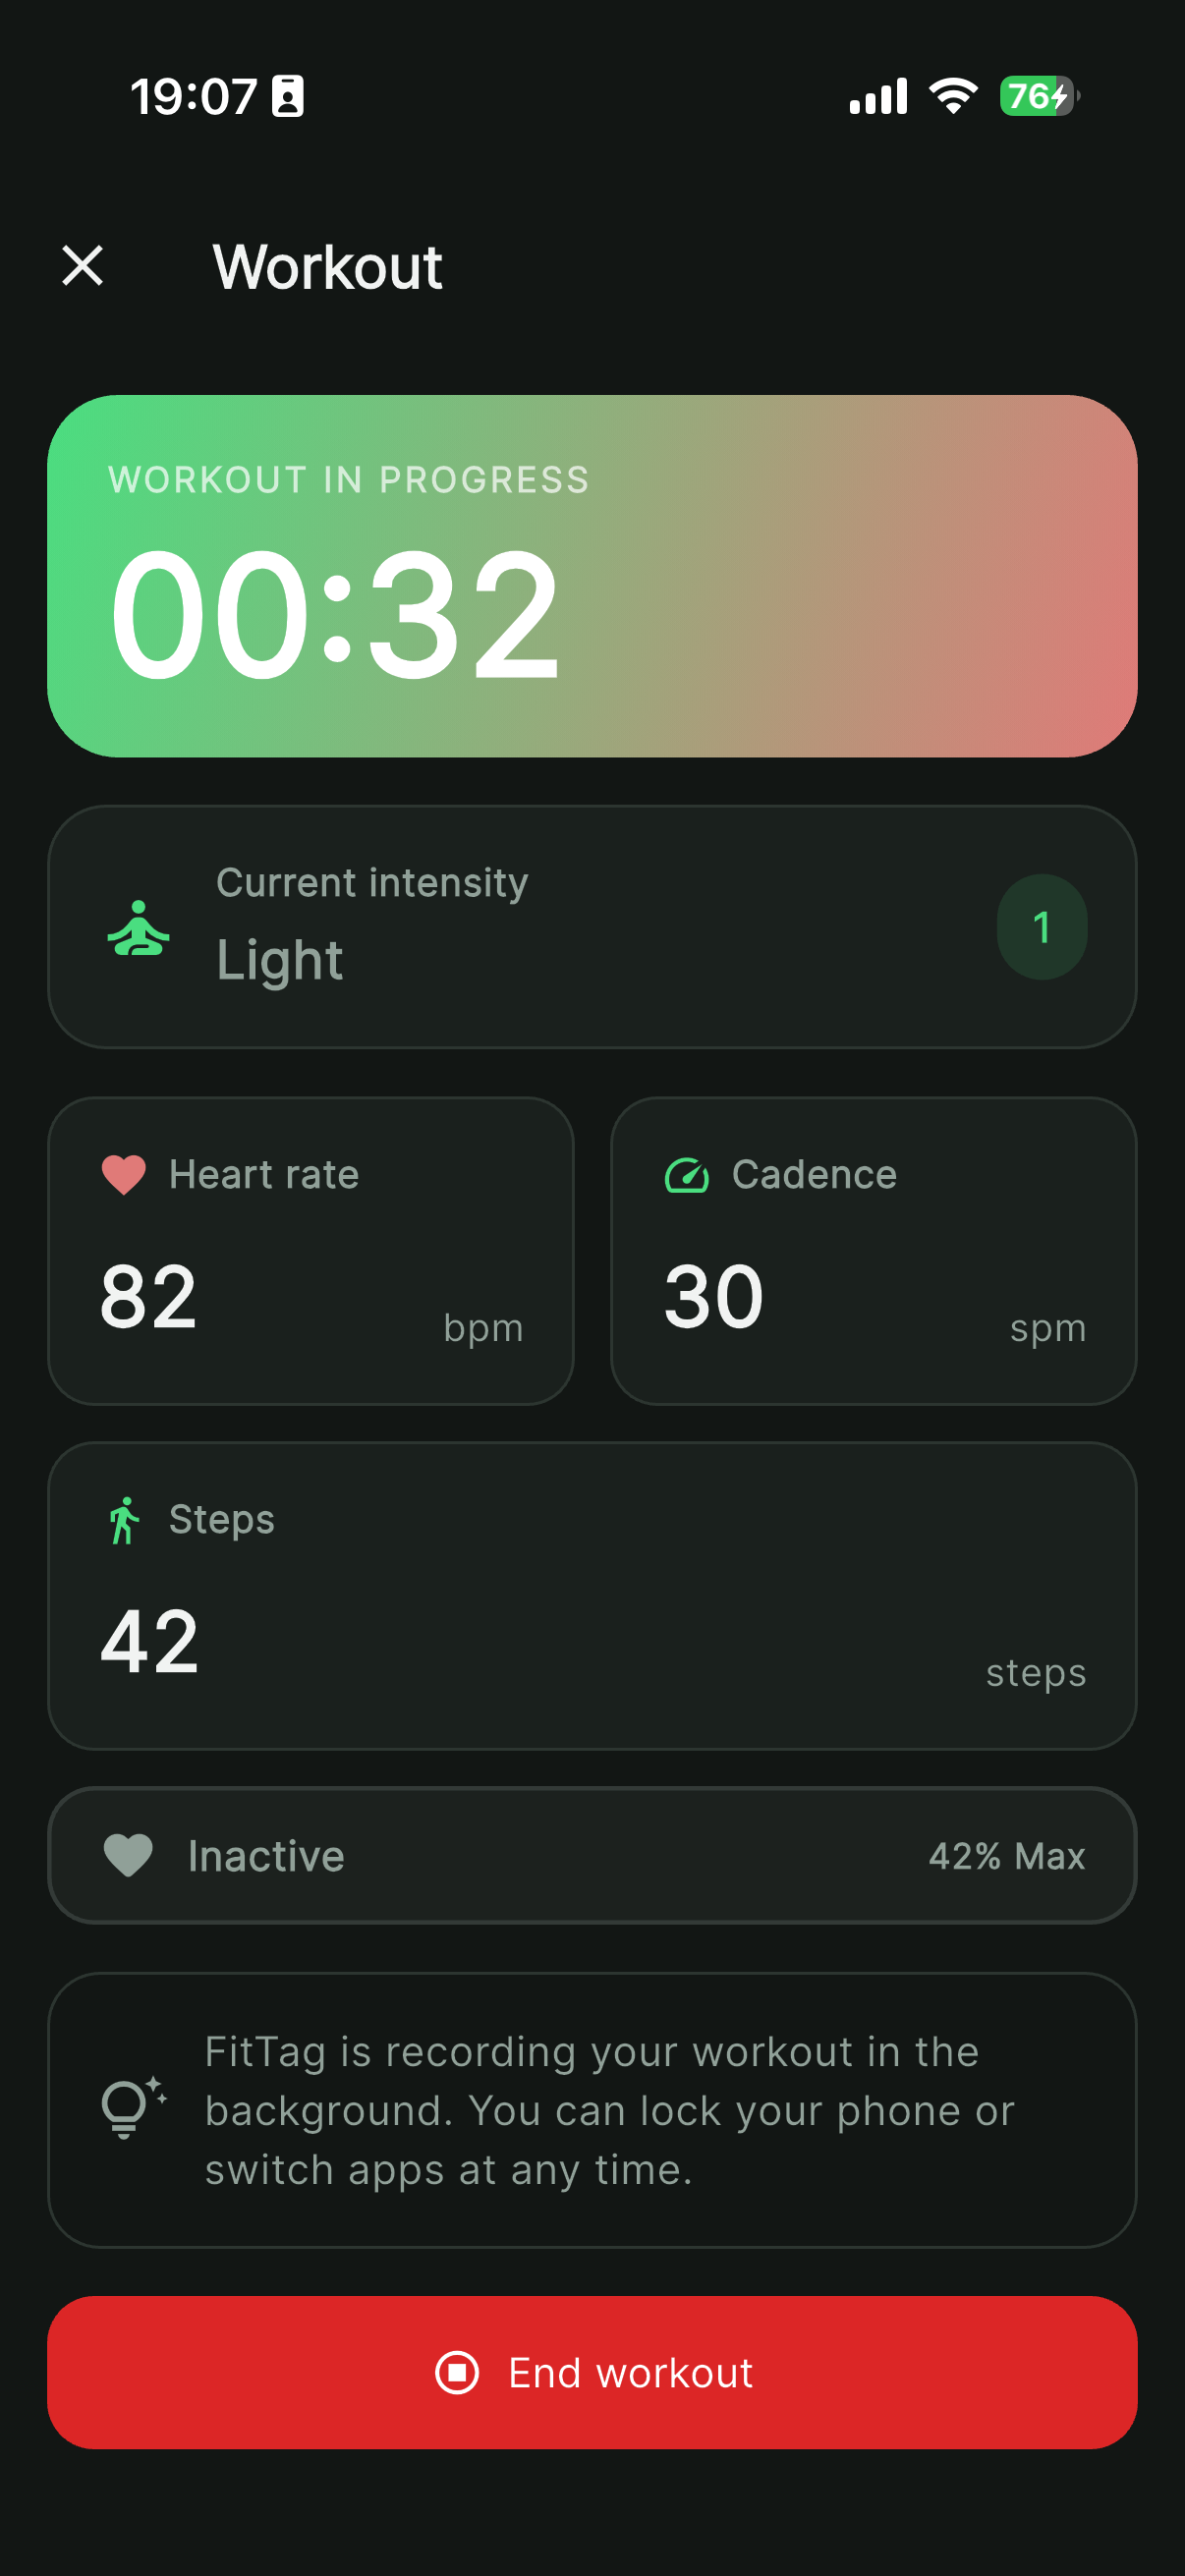
\includegraphics[width=\textwidth]{img/app/workout_screen.png}
        \caption{Allenamento attivo}
        \label{fig:workout_active}
    \end{subfigure}
    \hfill
    \begin{subfigure}[t]{0.3\textwidth}
        \centering
        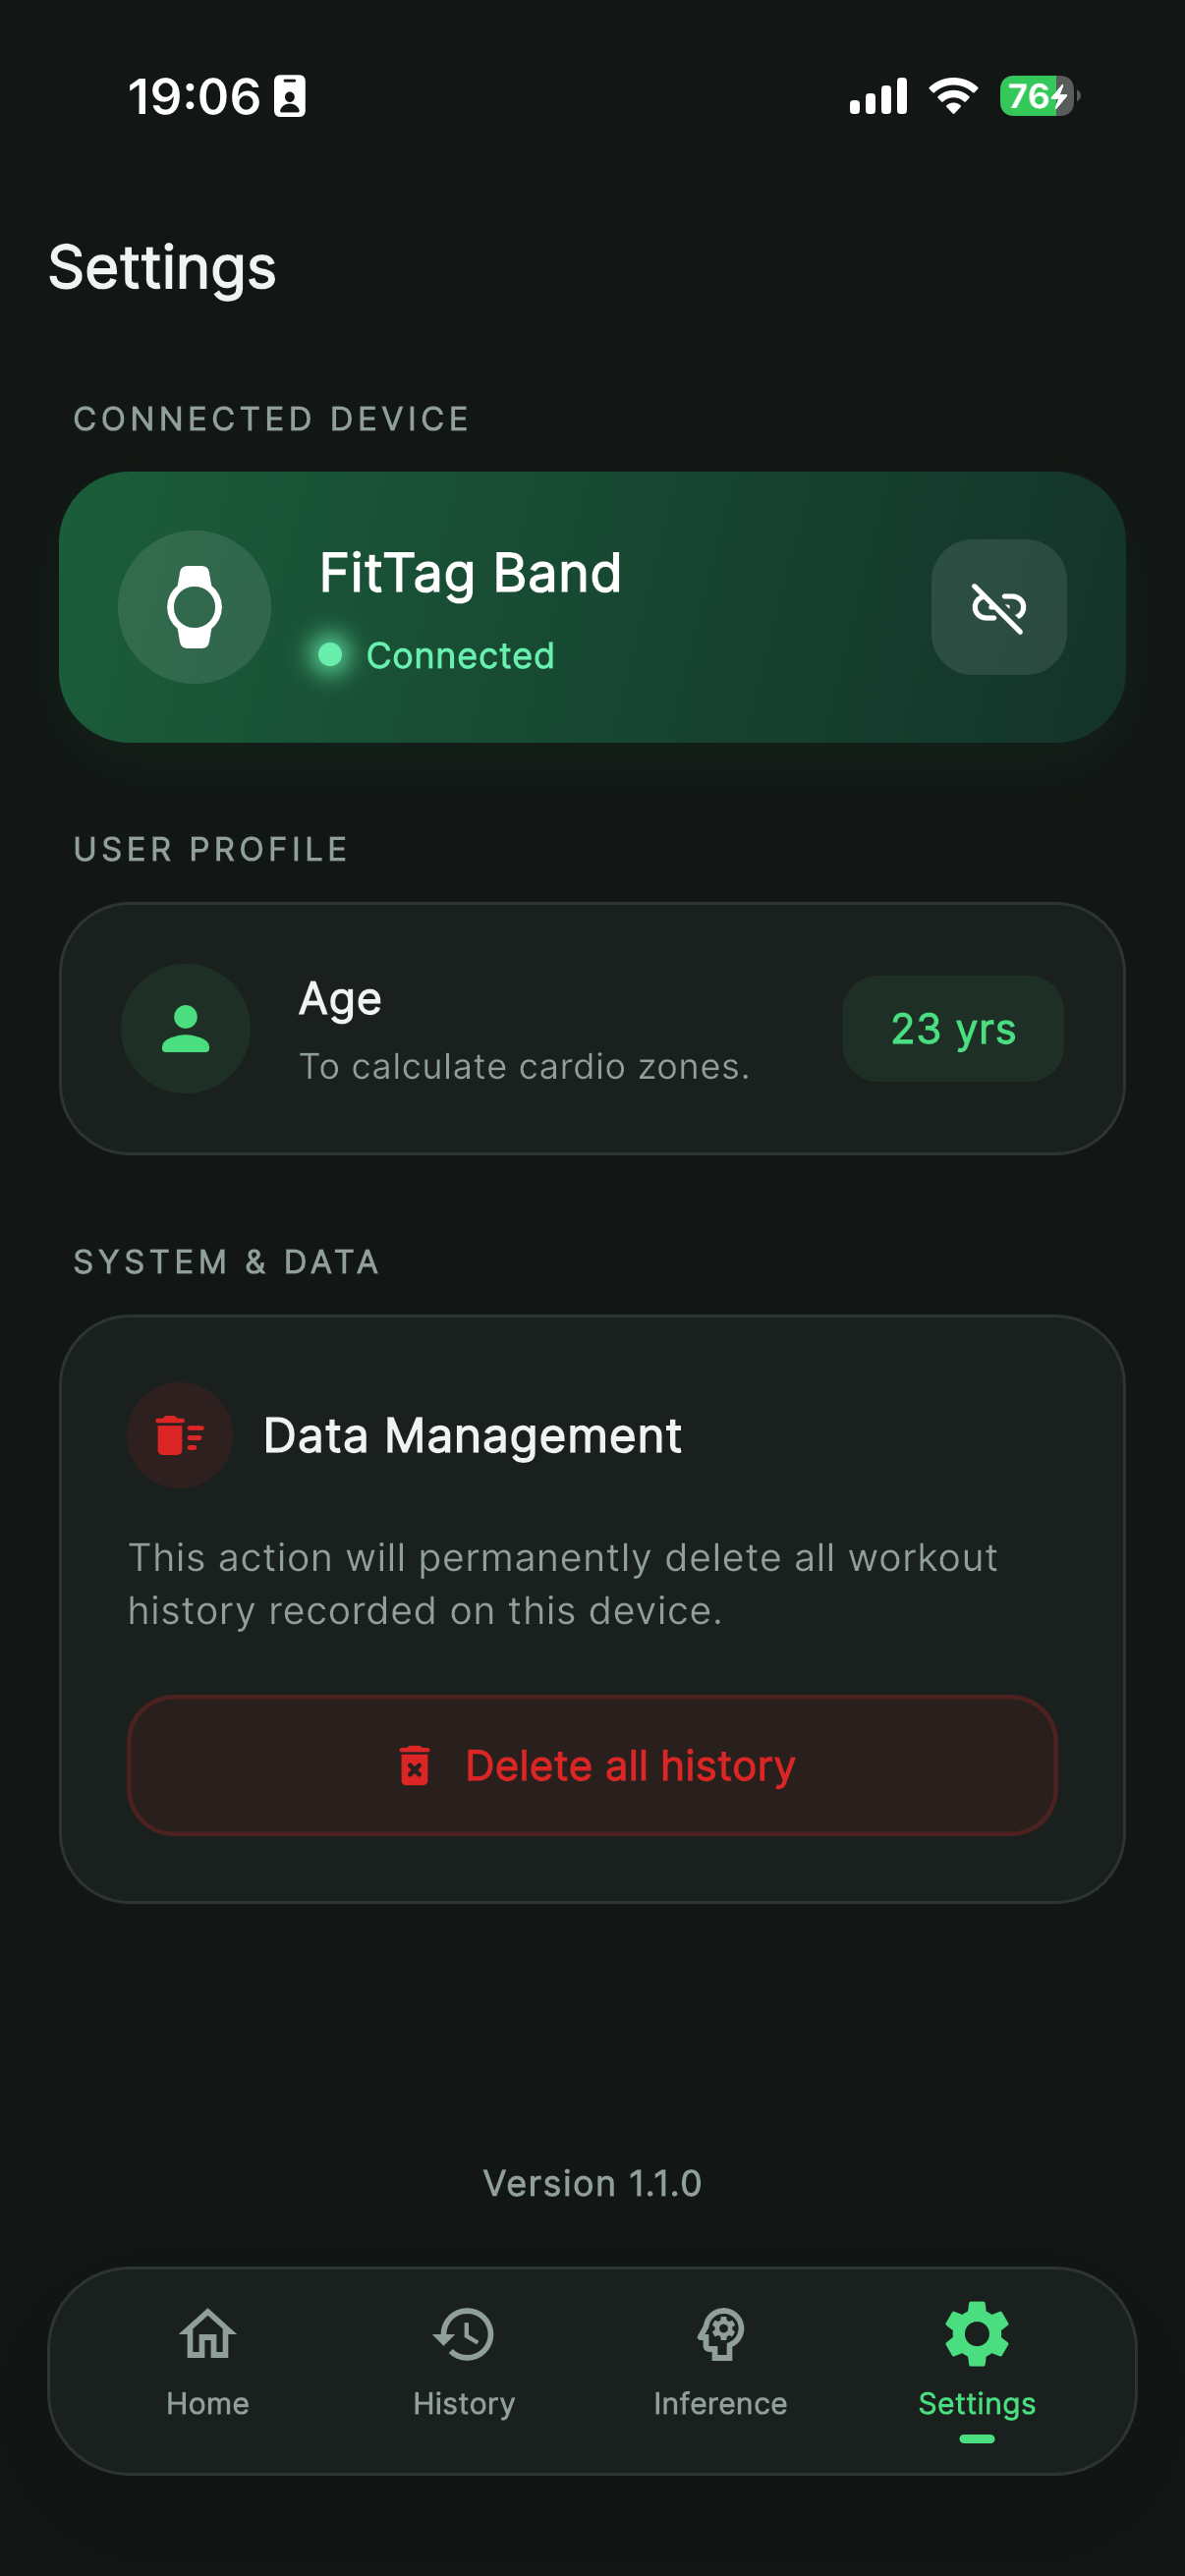
\includegraphics[width=\textwidth]{img/app/settings_screen.png}
        \caption{Impostazioni}
        \label{fig:settings_screen}
    \end{subfigure}
    \caption{Schermate dell'applicazione FitTag App.}
    \label{fig:app_screens}
\end{figure}

\section{Protocollo di comunicazione BLE}
L'interazione tra l'applicazione companion e il bracciale FitTag Band avviene attraverso lo stack protocollare Bluetooth Low Energy (BLE), in cui lo smartphone assume il ruolo di \textit{GATT Client} e il wearable funge da \textit{GATT Server}. Questo modello di comunicazione asincrono consente di minimizzare il tempo di attivazione del modulo radio, riducendo drasticamente il consumo energetico di entrambi i dispositivi.

La scoperta del bracciale avviene tramite una scansione wireless mirata, implementata all'interno del metodo \texttt{scanForDevices()} del servizio \texttt{FitTagBleService}. Per evitare di mostrare all'utente una lista congestionata da altri dispositivi Bluetooth circostanti (quali auricolari o smart TV), l'app applica un filtro di scansione basato esclusivamente sul \textbf{Service UUID} custom esposto dal firmware (\texttt{19b10000-e8f2-537e-4f6c-d104768a1214}). Una volta agganciato il dispositivo prescelto, il client avvia il processo di \textit{Service Discovery} per mappare le caratteristiche GATT esposte. Le caratteristiche operative utilizzate per coordinare lo scambio dati e la sincronizzazione dello stato sono descritte dettagliatamente nella Tabella~\ref{tab:ble_characteristics}.

\begin{table}[ht]
    \centering
    \small
    \renewcommand{\arraystretch}{1.4}
    \begin{tabular}{>{\raggedright\arraybackslash}p{4.2cm} >{\raggedright\arraybackslash}p{2.0cm} >{\raggedright\arraybackslash}p{6.6cm}}
        \hline
        \textbf{Caratteristica / UUID} & \textbf{Proprietà} & \textbf{Descrizione operativa} \\ \hline
        \texttt{ctrlChar} \newline {\tiny\texttt{19b10001-\allowbreak e8f2-\allowbreak 537e-\allowbreak 4f6c-\allowbreak d104768a1214}} & Scrittura, Lettura & Utilizzata per l'invio di comandi di cambio stato (payload a singolo byte). Consente all'applicazione di controllare la macchina a stati del bracciale. \\ \hline
        \texttt{dataLogChar} \newline {\tiny\texttt{19b10002-\allowbreak e8f2-\allowbreak 537e-\allowbreak 4f6c-\allowbreak d104768a1214}} & Notifica & Trasmissione ad alta frequenza dei dati dei sensori inerziali grezzi (accelerometro e giroscopio), impiegata per la calibrazione e la raccolta dati. \\ \hline
        \texttt{workoutChar} \newline {\tiny\texttt{19b10003-\allowbreak e8f2-\allowbreak 537e-\allowbreak 4f6c-\allowbreak d104768a1214}} & Notifica & Canale per la notifica dei dati elaborati (frequenza cardiaca, passi, cadenza, livello di sforzo) durante la sessione di allenamento. \\ \hline
        \texttt{inferChar} \newline {\tiny\texttt{19b10004-\allowbreak e8f2-\allowbreak 537e-\allowbreak 4f6c-\allowbreak d104768a1214}} & Notifica & Invio in tempo reale delle predizioni dell'attività calcolate dal modello di classificazione a bordo del bracciale. \\ \hline
        \texttt{batteryLevelChar} \newline {\tiny\texttt{00002a19-\allowbreak 0000-\allowbreak 1000-\allowbreak 8000-\allowbreak 00805f9b34fb}} & Lettura & Caratteristica dello standard Battery Service che espone la percentuale di carica residua della batteria del wearable. \\ \hline
    \end{tabular}
    \caption{Mappatura delle caratteristiche del protocollo GATT BLE di FitTag.}
    \label{tab:ble_characteristics}
\end{table}

\subsection{Gestione delle transizioni di stato}
La macchina a stati finiti (FSM) che regola il funzionamento del bracciale è progettata per preservare l'hardware e ottimizzare i consumi. Per questo motivo, il dispositivo non consente il passaggio diretto tra due modalità attive (como ad esempio passare direttamente dalla modalità di allenamento a quella di inferenza). Qualsiasi transizione tra le diverse modalità operative deve obbligatoriamente passare per lo stato di riposo, denominato \texttt{IDLE\_STATE}.

A livello software, l'applicazione gestisce questa limitazione coordinando una sequenza temporizzata per ogni cambio di stato:
\begin{enumerate}
    \item L'applicazione invia al bracciale un comando per forzare il ritorno allo stato di riposo.
    \item L'applicazione attende una brevissima pausa di assestamento di circa $150ms$. Questo intervallo consente al dispositivo di spegnere i moduli hardware precedentemente attivi e prepararsi alla ricezione di una nuova modalità.
    \item Viene inviato il comando per attivare lo stato di destinazione desiderato.
\end{enumerate}
Questo meccanismo sequenziale previene eventuali blocchi o conflitti di configurazione a livello dei sensori del bracciale, garantendo la stabilità del collegamento wireless.

\subsection{Verifica periodica della connessione}
A causa della natura del collegamento wireless, il bracciale può allontanarsi o disconnettersi senza che il sistema operativo del telefono segnali immediatamente l'evento. Per evitare che l'applicazione mostri il bracciale come connesso quando in realtà non lo è, è stato implementato un meccanismo di controllo periodico della connessione che opera con due logiche distinte:
\begin{itemize}
    \item \textbf{In stato di riposo:} L'applicazione esegue una lettura periodica del livello di batteria ogni $4$ secondi. Se questa comunicazione fallisce o non risponde entro un certo limite di tempo, il collegamento viene considerato interrotto e l'applicazione aggiorna lo stato dell'interfaccia utente a disconnesso.
    \item \textbf{In stato di trasmissione attiva (allenamento o inferenza):} Poiché il bracciale invia già dati in modo continuo, l'applicazione verifica semplicemente la regolarità della ricezione di questi pacchetti. Se non si ricevono aggiornamenti per più di $5$ secondi consecutivi, l'applicazione rileva la perdita del segnale, interrompe la sessione attiva salvando i dati parziali accumulati e si riconnette in stato disconnesso.
\end{itemize}

\subsection{Diagramma di sequenza delle interazioni}
Per comprendere appieno come l'applicazione e la smart band si scambino informazioni e coordinino i propri stati interni, il diagramma di sequenza in Figura~\ref{fig:diagramma_sequenza} illustra graficamente i messaggi GATT scambiati lungo il canale BLE nelle tre modalità operative principali dell'ecosistema.

\begin{figure}[ht]
    \centering
    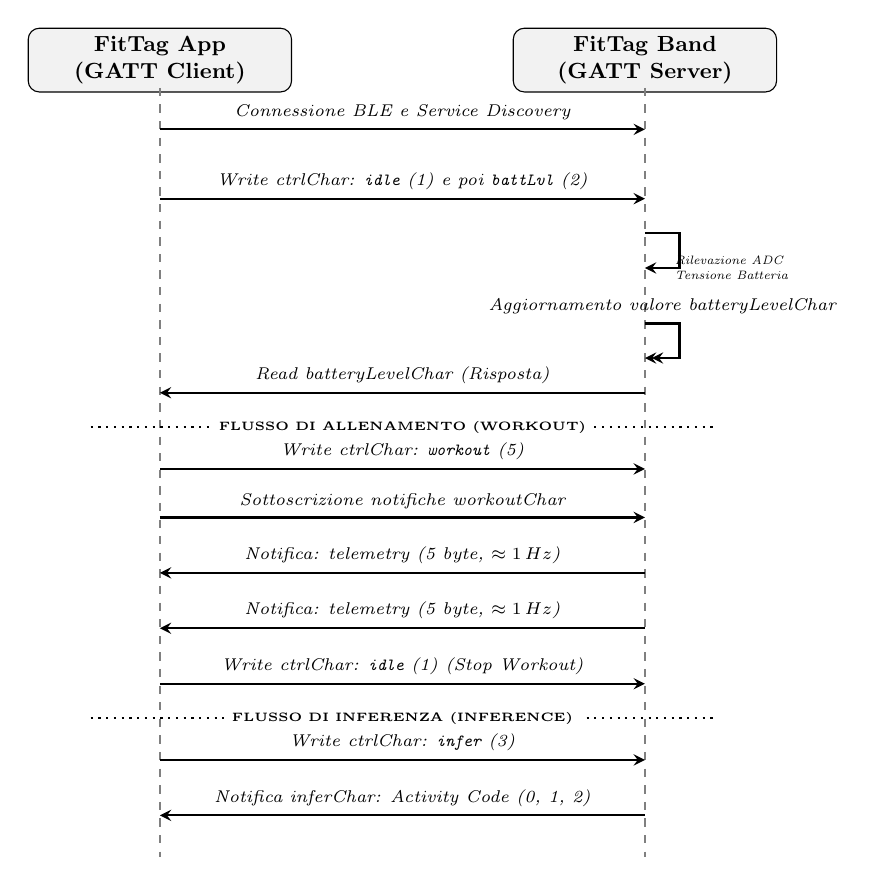
\begin{tikzpicture}[>=stealth, scale=0.88, every node/.style={transform shape}]
        % Box styles
        \tikzset{
            box/.style={draw, rectangle, rounded corners, fill=gray!10, minimum width=3.8cm, minimum height=0.8cm, font=\bfseries\small, align=center},
            lbl/.style={font=\scriptsize\itshape, align=center},
            msg/.style={->, thick},
            state/.style={draw, rectangle, fill=green!10, minimum width=2.5cm, minimum height=0.5cm, font=\tiny\ttfamily, align=center}
        }
        
        % Vertical Lifelines
        \node[box] (app) at (0, 0) {FitTag App\\(GATT Client)};
        \node[box] (band) at (7, 0) {FitTag Band\\(GATT Server)};
        
        \draw[dashed, thick, gray] (0, -0.4) -- (0, -11.5);
        \draw[dashed, thick, gray] (7, -0.4) -- (7, -11.5);
        
        % Phase 1: Connection & Battery
        \draw[msg] (0, -1) -- node[above, lbl] {Connessione BLE e Service Discovery} (7, -1);
        \draw[msg] (0, -2) -- node[above, lbl] {Write ctrlChar: \texttt{idle} (1) e poi \texttt{battLvl} (2)} (7, -2);
        
        % Band self loop/state
        \draw[thick] (7, -2.5) -- (7.5, -2.5) -- (7.5, -3) -- node[right, font=\tiny\itshape, align=left] {Rilevazione ADC\\Tensione Batteria} (7.1, -3);
        \draw[msg] (7.1, -3) -- (7, -3);
        
        \draw[msg] (7, -3.8) -- node[above, lbl] {Aggiornamento valore batteryLevelChar} (7.5, -3.8) -- (7.5, -4.3) -- (7.1, -4.3);
        \draw[msg] (7.1, -4.3) -- (7, -4.3);
        
        \draw[msg] (7, -4.8) -- node[above, lbl] {Read batteryLevelChar (Risposta)} (0, -4.8);
        
        % Separator
        \draw[dotted, thick] (-1, -5.3) -- (8, -5.3) node[pos=0.5, fill=white, font=\tiny\bfseries] {FLUSSO DI ALLENAMENTO (WORKOUT)};
        
        % Phase 2: Workout
        \draw[msg] (0, -5.9) -- node[above, lbl] {Write ctrlChar: \texttt{workout} (5)} (7, -5.9);
        \draw[msg] (0, -6.6) -- node[above, lbl] {Sottoscrizione notifiche workoutChar} (7, -6.6);
        \draw[msg] (7, -7.4) -- node[above, lbl] {Notifica: telemetry (5 byte, $\approx 1\,\text{Hz}$)} (0, -7.4);
        \draw[msg] (7, -8.2) -- node[above, lbl] {Notifica: telemetry (5 byte, $\approx 1\,\text{Hz}$)} (0, -8.2);
        \draw[msg] (0, -9.0) -- node[above, lbl] {Write ctrlChar: \texttt{idle} (1) (Stop Workout)} (7, -9.0);
        
        % Separator
        \draw[dotted, thick] (-1, -9.5) -- (8, -9.5) node[pos=0.5, fill=white, font=\tiny\bfseries] {FLUSSO DI INFERENZA (INFERENCE)};
        
        % Phase 3: Inference
        \draw[msg] (0, -10.1) -- node[above, lbl] {Write ctrlChar: \texttt{infer} (3)} (7, -10.1);
        \draw[msg] (7, -10.9) -- node[above, lbl] {Notifica inferChar: Activity Code (0, 1, 2)} (0, -10.9);
        
    \end{tikzpicture}
    \caption{Diagramma di sequenza delle interazioni GATT BLE tra FitTag App e FitTag Band.}
    \label{fig:diagramma_sequenza}
\end{figure}

Il flusso di messaggi si articola in tre macro-fasi sequenziali o alternative:
\begin{enumerate}
    \item \textbf{Inizializzazione e sincronizzazione batteria:} all'avvio del collegamento, l'app interroga la periferica. Per leggere la carica residua, viene eseguito l'instradamento passante per lo stato di riposo (\texttt{idle}) prima di scrivere \texttt{battLvl} (2). Il bracciale campiona la tensione della batteria tramite l'ADC integrato, scrive la percentuale stimata sulla caratteristica standard del \textit{Battery Level} (\texttt{0x2A19}) e si rimette in standby autonomamente. L'app esegue quindi una lettura sincrona sulla medesima caratteristica per aggiornare l'interfaccia.
    \item \textbf{Sessione di allenamento (workout):} alla pressione del tasto di avvio, l'applicazione ordina la transizione del bracciale allo stato \texttt{workout} (5) e si iscrive alle notifiche del canale \texttt{workoutChar}. Da questo momento, il bracciale campiona attivamente la frequenza cardiaca ed i passi tramite i sensori integrati, trasmettendo pacchetti di telemetria da 5 byte a cadenza regolare ($\approx 1\,\text{Hz}$) fino a quando l'utente non interrompe la sessione riportando il dispositivo a riposo.
    \item \textbf{Classificazione edge AI (inference):} quando l'utente naviga sulla schermata di inferenza, l'app richiede lo stato \texttt{infer} (3). La band esegue l'HAR a bordo e invia notifiche asincrone su \texttt{inferChar} contenenti gli indici delle attività (0 per riposo, 1 per camminata, 2 per corsa), che vengono decodificate dall'applicazione per sincronizzare la pulsazione delle icone della UI.
\end{enumerate}

\section{Interfaccia utente}

\subsection{Schermata principale}
La schermata Home (Figura~\ref{fig:home_screen}) rappresenta il punto di ingresso principale dell'utente. Essa è progettata secondo canoni estetici moderni, riflettendo l'identità visiva dell'ecosistema FitTag. 
Il widget principale è una card dotata di un gradiente cromatico dinamico: quando il bracciale è connesso, la card assume una tonalità verde smeraldo brillante, mentre in caso di disconnessione assume una colorazione marrone scuro, fornendo un feedback visivo immediato.

All'apertura della schermata Home, l'applicazione (se connessa al FitTag Band) avvia automaticamente il processo di sincronizzazione del livello della batteria. 
Questo flusso richiede un coordinamento specifico per via del funzionamento hardware descritto:
\begin{enumerate}
    \item L'app richiede la transizione passante per l'idle, ponendo il bracciale in \texttt{BATT\_LVL\_STATE} (2).
    \item Il firmware del bracciale si risveglia, abilita il convertitore analogico-digitale (ADC), campiona la tensione presente sui pin di alimentazione, calcola la percentuale stimata, scrive tale valore all'interno della caratteristica standard del \textit{Battery Level} e ritorna automaticamente in \texttt{IDLE}.
    \item L'applicazione attende un tempo di campionamento stimato in $700ms$, dopodiché interroga in lettura il Battery Service standard memorizzando la percentuale letta.
\end{enumerate}
Il livello della batteria viene mostrato graficamente con icone incrementali. La schermata Home ospita inoltre le statistiche aggregate ricavate dallo storico e il pulsante per avviare un nuovo allenamento.

\subsection{Schermata di allenamento}
Quando l'utente avvia un allenamento, l'applicazione forza la transizione del bracciale in \texttt{WORKOUT\_STATE} (5) ed effettua la sottoscrizione ai messaggi di notifica della caratteristica \texttt{workoutChar}. Le letture avvengono con una cadenza di circa $1\,\text{Hz}$. Ciascun pacchetto dati trasmesso dal bracciale ha una dimensione di esattamente \textbf{5 byte}. L'applicazione decodifica il pacchetto binario ricevuto per ricostruire le seguenti metriche:
\begin{itemize}
    \item \textbf{Byte 0 (BPM):} Frequenza cardiaca istantanea estratta come intero a 8 bit senza segno.
    \item \textbf{Byte 1 e 2 (passi):} Conto totale dei passi accumulati. Trattandosi di un valore a 16 bit trasmesso con codifica Little-endian, l'app lo decodifica combinando i byte mediante l'operazione:
    \begin{equation}
        \text{totalSteps} = \text{bytes}[1] \mid (\text{bytes}[2] \ll 8)
    \end{equation}
    dove il byte in posizione 1 rappresenta i bit meno significativi (LSB) e il byte in posizione 2 i bit più significativi (MSB).
    \item \textbf{Byte 3 (cadenza):} Cadenza istantanea di camminata/corsa in passi al minuto (SPM).
    \item \textbf{Byte 4 (intensità):} Livello di intensità dello sforzo (valore discreto da 1 a 10).
\end{itemize}
La schermata di allenamento attivo (Figura~\ref{fig:workout_active}) presenta un cronometro centrale che traccia la durata della sessione. Per rendere la lettura immediata durante lo sforzo fisico, il livello di intensità viene categorizzato cromaticamente in tre fasce: \textit{Light} (1--3, verde), \textit{Moderate} (4--7, giallo/arancione) ed \textit{Intense} (8--10, rosso).

\paragraph{Tracciamento delle zone cardio:} 
Durante l'allenamento attivo, l'app calcola in tempo reale la zona di frequenza cardiaca corrente dell'utente per fornire un feedback visivo immediato sullo sforzo cardiovascolare. Il calcolo si basa sulla frequenza cardiaca massima ($\text{FC}_{\text{max}}$) stimata tramite la formula classica:
\begin{equation}
    \text{FC}_{\text{max}} = 220 - \text{età}
\end{equation}
L'età viene recuperata dal profilo utente (impostata di default a 30 anni se non configurata). 
In base al rapporto percentuale tra la frequenza cardiaca istantanea ed il valore $\text{FC}_{\text{max}}$, lo sforzo viene suddiviso in cinque zone di allenamento, mostrate graficamente tramite un indicatore colorato:
\begin{itemize}
    \item \textbf{Inattivo (sotto il 50\%):} stato a riposo (colore grigio).
    \item \textbf{Riscaldamento (50\%--60\%):} riscaldamento e recupero attivo (colore blu).
    \item \textbf{Brucia grassi (60\%--70\%):} andatura aerobica leggera per il consumo lipidico (colore verde).
    \item \textbf{Aerobica (70\%--80\%):} andatura aerobica moderata per il miglioramento della resistenza (colore arancione).
    \item \textbf{Anaerobica (80\%--90\%):} sforzo anaerobico intenso per lo sviluppo della soglia lattacida (colore arancione scuro).
    \item \textbf{Massimo sforzo (oltre il 90\%):} sforzo massimale ad alta intensità (colore rosso).
\end{itemize}
Alla pressione del tasto di arresto, l'app rimuove la sottoscrizione alle notifiche, ordina alla band di tornare in \texttt{IDLE}, impacchetta la serie temporale accumulata e la scrive in formato JSON.

\subsection{Dettaglio dell'allenamento}
Selezionando una sessione di allenamento salvata, l'interfaccia utente mostra una schermata di dettaglio analitico (Figura~\ref{fig:workout_detail_screen}). L'app analizza l'intero vettore delle serie temporali dei dati registrati per estrarre informazioni aggregate: il battito cardiaco medio e massimo, la cadenza media e quella di picco, e il profilo temporale dell'intensità dello sforzo.

I dati vengono plottati su quattro grafici a linee indipendenti tramite la libreria \texttt{fl\_chart}:
\begin{itemize}
    \item \textbf{Battito cardiaco:} Mostra la risposta cardiaca dell'utente nel tempo.
    \item \textbf{Passi accumulati:} Evidenzia la progressione del conteggio passi.
    \item \textbf{Cadenza:} Traccia l'andamento della frequenza di passo, utile per analizzare la regolarità del passo.
    \item \textbf{Intensità:} Visualizza la variazione dell'intensità dello sforzo durante le diverse fasi della sessione.
\end{itemize}
Per garantire una resa grafica eccellente anche per sessioni brevi (con pochi punti di telemetria reali), l'applicazione implementa una logica di interpolazione dinamica che modella i punti intermedi applicando funzioni sinusoidali con fluttuazioni casuali per simulare l'andamento fisiologico reale dei parametri. Ciascun grafico supporta interazioni touch per esplorare i singoli campioni tramite tooltip e formatta l'asse delle ascisse calcolando il tempo trascorso relativo in minuti e secondi (\texttt{MM:SS}).

\paragraph{Scomposizione delle zone cardio storiche:}
Oltre ai grafici a linee, la schermata di dettaglio include una card riassuntiva dedicata all'analisi delle zone di frequenza cardiaca. 
L'applicazione elabora l'intera serie temporale della frequenza cardiaca registrata durante la sessione e calcola il tempo totale speso (espresso in minuti e secondi) e la relativa percentuale per ciascuna delle cinque zone cardio. 
Questi dati vengono visualizzati attraverso un elenco descrittivo affiancato da barre di progresso colorate associate cromaticamente alle rispettive zone, offrendo un quadro immediato della ripartizione fisiologica dell'allenamento dell'utente.

\begin{figure}[ht]
    \centering
    \begin{subfigure}[t]{0.3\textwidth}
        \centering
        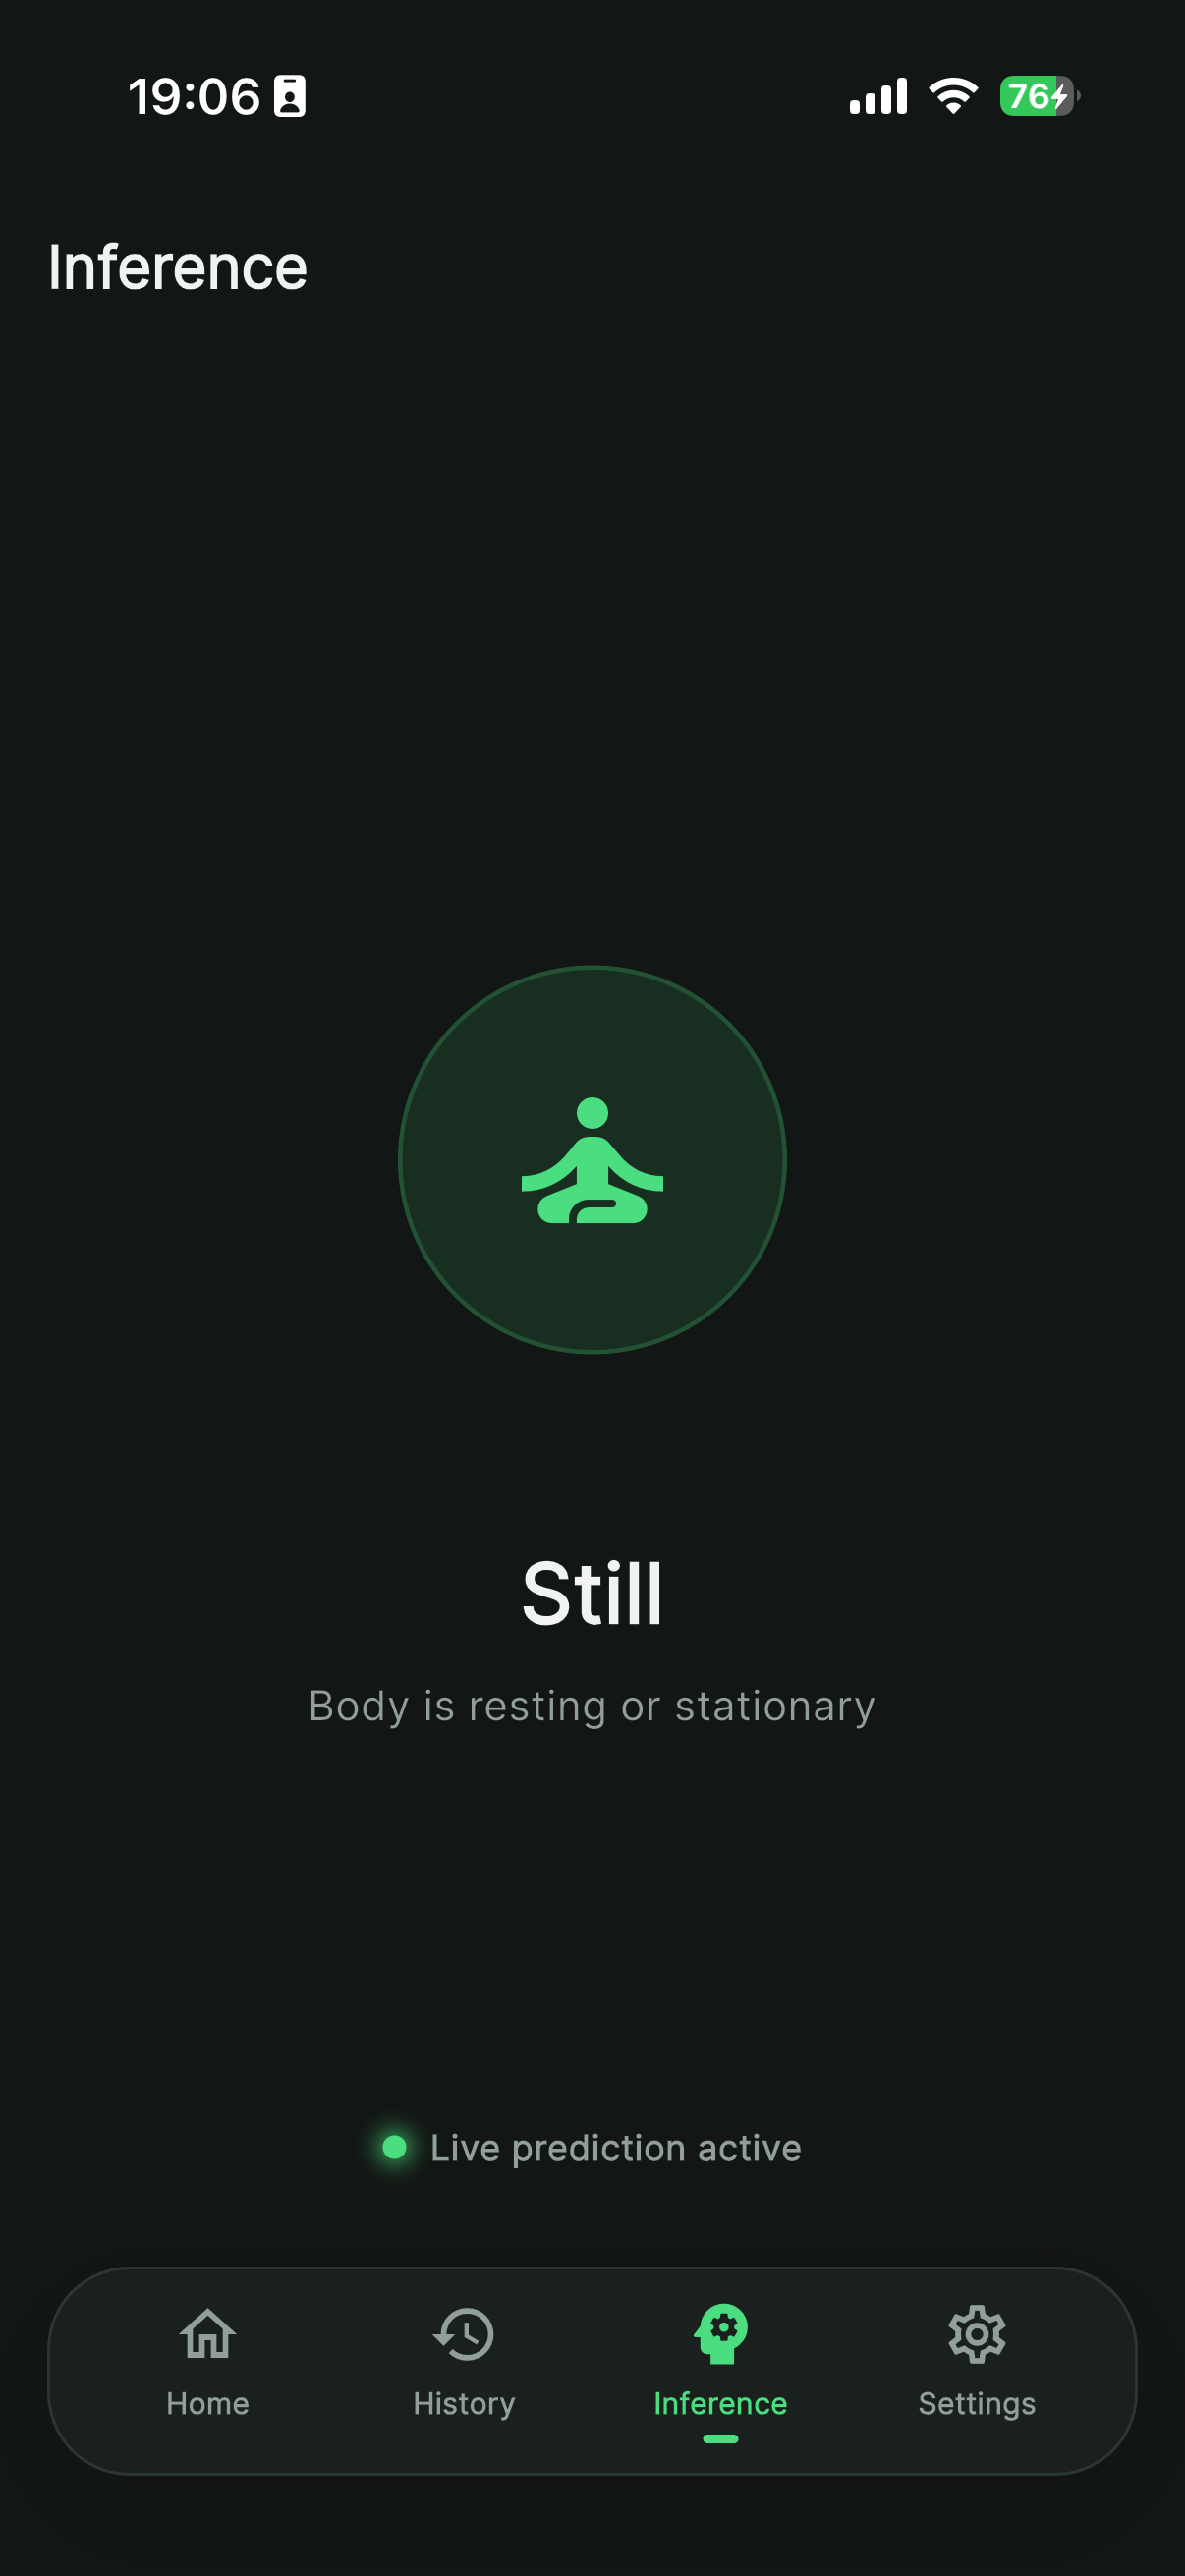
\includegraphics[width=\textwidth]{img/app/inference_screen.png}
        \caption{Schermata di inferenza}
        \label{fig:inference_screen}
    \end{subfigure}
    \hspace{1cm}
    \begin{subfigure}[t]{0.3\textwidth}
        \centering
        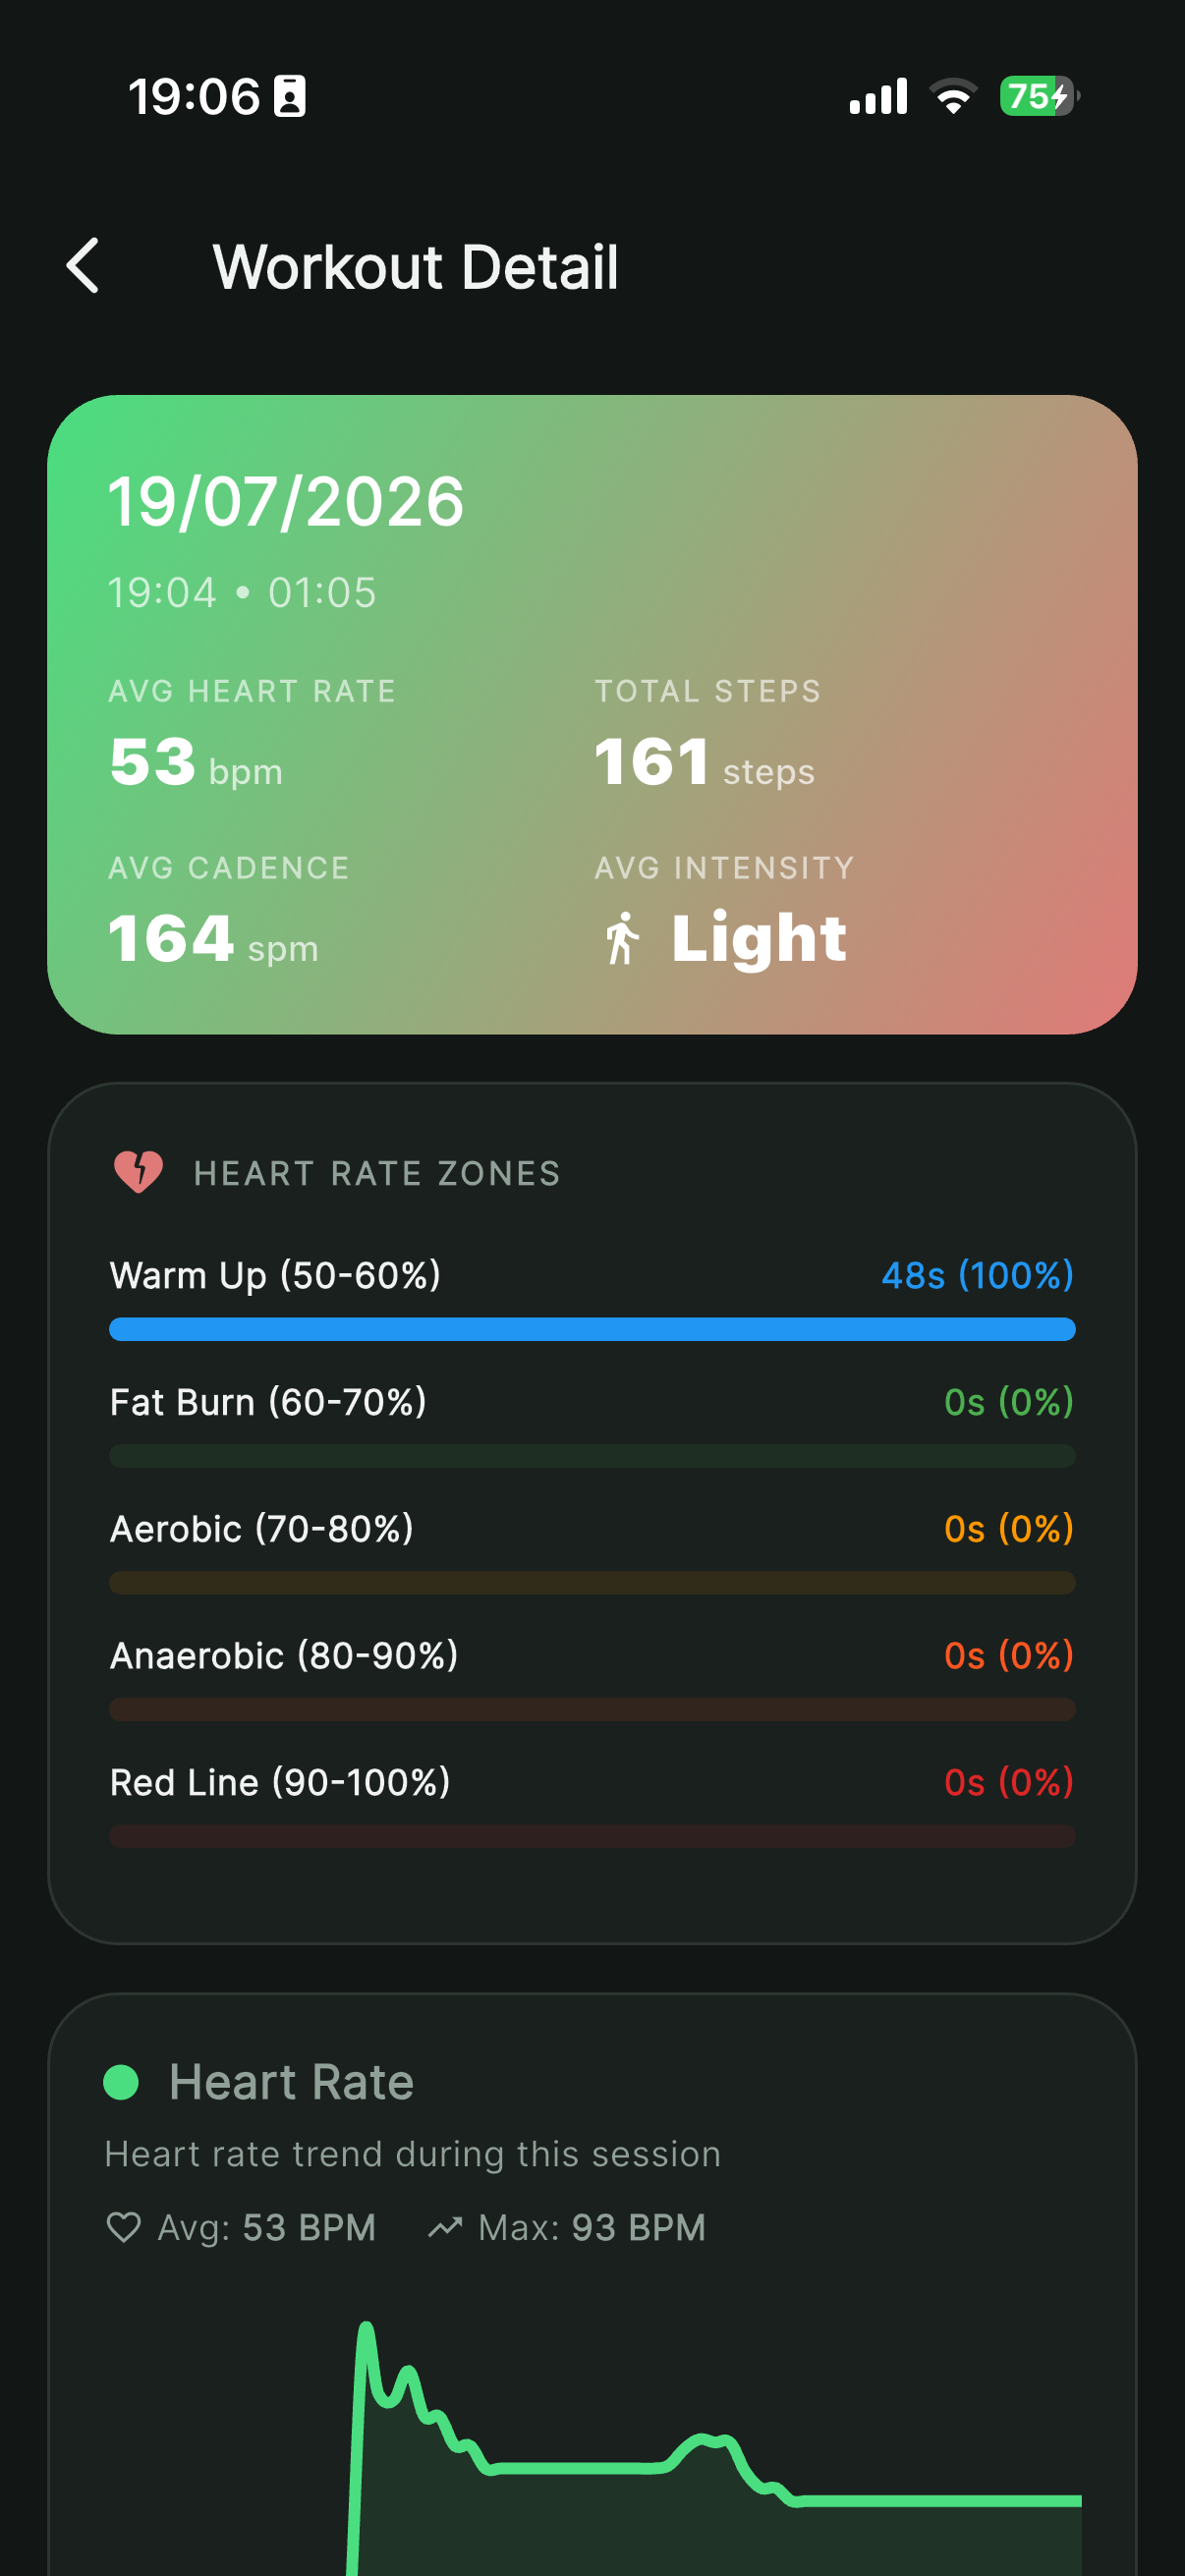
\includegraphics[width=\textwidth]{img/app/workout_detail_screen.png}
        \caption{Grafici di dettaglio allenamento}
        \label{fig:workout_detail_screen}
    \end{subfigure}
    \caption{Visualizzazioni dell'inferenza in tempo reale ed analisi dei grafici temporali.}
\end{figure}

\subsection{Schermata di inferenza}
La schermata di inferenza (Figura~\ref{fig:inference_screen}) permette di visualizzare direttamente i risultati delle predizioni del classificatore Random Forest operante sul firmware del bracciale. 
Per prevenire l'usura della batteria del wearable causata dall'esecuzione continuativa dell'algoritmo di Machine Learning a bordo chip e dal campionamento ad alta frequenza dei sensori inerziali, l'applicazione applica una politica di attivazione rigorosa basata sul ciclo di vita della schermata:
\begin{itemize}
    \item \textbf{Fase di inizializzazione:} all'apertura della pagina, l'applicazione richiede la transizione del bracciale allo stato di inferenza e sottoscrive il flusso di notifiche per ricevere le predizioni.
    \item \textbf{Fase di chiusura:} non appena l'utente decide di navigare verso un'altra schermata o di chiudere l'applicazione, quest'ultima interrompe la ricezione dei dati e invia immediatamente una richiesta per riportare il bracciale nello stato di riposo, spegnendo i sensori inerziali.
\end{itemize}

I codici numerici inviati dal bracciale su \texttt{inferChar} vengono decodificati in tempo reale dall'applicazione per aggiornare l'interfaccia utente:
\begin{itemize}
    \item \textbf{Classe 0 (Still):} corpo a riposo o stazionario. L'applicazione mostra un'icona statica di rilassamento. Non viene applicata alcuna animazione alla cornice circostante.
    \item \textbf{Classe 1 (Walking):} camminata regolare. L'app mostra un'icona di persona che cammina. La cornice dell'icona avvia un'animazione di pulsazione concentrica lenta.
    \item \textbf{Classe 2 (Running):} corsa o movimento rapido. L'app mostra un'icona di persona che corre. Per rispecchiare l'elevato ritmo motorio, la pulsazione grafica della cornice viene accelerata.
\end{itemize}
Questo meccanismo di variazione dinamica della frequenza di pulsazione visiva fornisce all'utente una percezione immediata della precisione del modello HAR, evidenziando come l'inferenza TinyML risponda prontamente ai cambi di andatura del soggetto.

\subsection{Schermata delle impostazioni}
La schermata \textit{Settings} (Figura~\ref{fig:settings_screen}) raggruppa le funzioni di connessione hardware e di gestione dello storage locale. 
Se l'app non è connessa a un bracciale, attiva una routine di scansione continua. I dispositivi rilevati vengono visualizzati in una lista ordinata in base alla potenza del segnale radio ricevuto.

L'applicazione decodifica il valore RSSI (\textit{Received Signal Strength Indicator}) in dBm per stimare la distanza fisica e la qualità del link radio, visualizzando un'icona del segnale colorata in tempo reale:
\begin{itemize}
    \item \textbf{Verde (RSSI $\ge -60\,\text{dBm}$):} segnale ottimale, accoppiamento stabile a breve distanza.
    \item \textbf{Giallo ($-70\,\text{dBm} \le \text{RSSI} < -60\,\text{dBm}$):} segnale buono, distanza moderata.
    \item \textbf{Arancione ($-85\,\text{dBm} \le \text{RSSI} < -70\,\text{dBm}$):} segnale debole, possibili rallentamenti di notifica.
    \item \textbf{Rosso (RSSI $< -85\,\text{dBm}$):} segnale stabile o a rischio per fuori portata.
\end{itemize}

\paragraph{Profilo utente ed impostazione dell'età:}
La schermata include una sezione dedicata al profilo utente, contenente una scheda per la gestione dell'età.
Cliccando sulla scheda, viene aperto un modale che permette all'utente di selezionare la propria età in un range compreso tra $10$ e $100$ anni.
Alla pressione del tasto di salvataggio, l'età selezionata viene persistita nel provider del servizio ed utilizzata per ricalcolare immediatamente le soglie percentuali delle zone cardio durante le sessioni di allenamento attive e nello storico.

\paragraph{Gestione dati locali:}
Infine, la schermata ospita la sezione di gestione della memoria locale. L'utente ha la possibilità di cancellare la cronologia degli allenamenti memorizzati. Trattandosi di un'operazione distruttiva, l'app implementa un flusso di sicurezza: la pressione del pulsante apre un modale personalizzato che spiega le conseguenze dell'operazione. Solo alla conferma esplicita dell'utente viene effettuata la pulizia dei dati in memoria.
